% Design of koblitz-s23-tuned-rho-20261015 (schematic; no data).
% Build: pdflatex design.tex; pdftoppm -png -r 160 -singlefile design.pdf design
\documentclass[border=6pt]{standalone}
\usepackage{tikz}
\usetikzlibrary{positioning,arrows.meta,fit}
\begin{document}
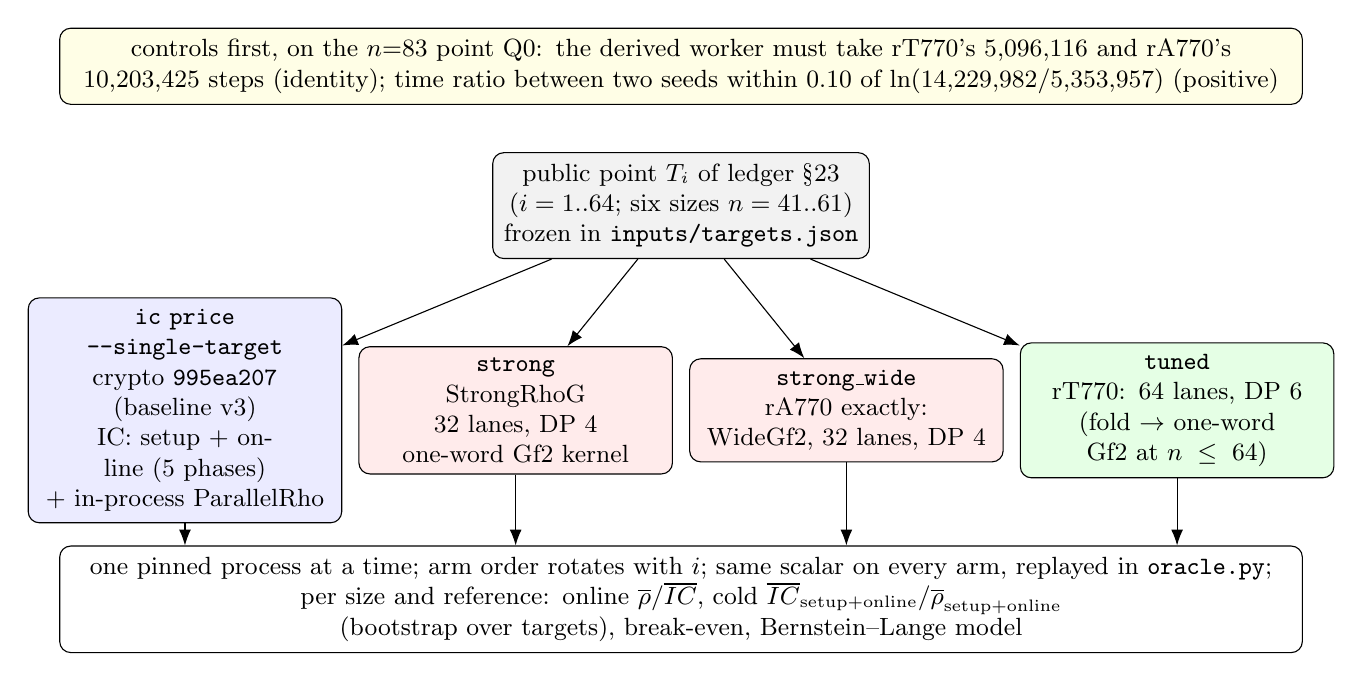
\begin{tikzpicture}[font=\small, box/.style={draw, rounded corners, align=center, inner sep=4pt},
  arr/.style={-{Latex[length=2mm]}}]
\node[box, fill=gray!10] (pt) at (0,0) {public point $T_i$ of ledger \S23\\($i=1..64$; six sizes $n=41..61$)\\frozen in \texttt{inputs/targets.json}};
\node[box, fill=blue!8, text width=3.7cm] (ic) at (-6.3,-2.6) {\texttt{ic price --single-target}\\crypto \texttt{995ea207} (baseline v3)\\IC: setup + online (5 phases)\\+ in-process ParallelRho};
\node[box, fill=red!8, text width=3.7cm] (st) at (-2.1,-2.6) {\texttt{strong}\\StrongRhoG 32 lanes, DP 4\\one-word Gf2 kernel};
\node[box, fill=red!8, text width=3.7cm] (sw) at (2.1,-2.6) {\texttt{strong\_wide}\\rA770 exactly:\\WideGf2, 32 lanes, DP 4};
\node[box, fill=green!10, text width=3.7cm] (tu) at (6.3,-2.6) {\texttt{tuned}\\rT770: 64 lanes, DP 6\\(fold $\to$ one-word Gf2 at $n\le64$)};
\foreach \x in {ic,st,sw,tu} \draw[arr] (pt) -- (\x);
\node[box, text width=15.5cm] (out) at (0,-5.0) {one pinned process at a time; arm order rotates with $i$; same scalar on every arm, replayed in \texttt{oracle.py};\\
per size and reference: online $\overline{\rho}/\overline{IC}$, cold $\overline{IC}_{\rm setup+online}/\overline{\rho}_{\rm setup+online}$ (bootstrap over targets), break-even, Bernstein--Lange model};
\foreach \x in {ic,st,sw,tu} \draw[arr] (\x.south) -- (\x.south |- out.north);
\node[box, fill=yellow!10, above=0.6cm of pt, text width=15.5cm] (ctl) {controls first, on the $n{=}83$ point Q0: the derived worker must take rT770's 5,096,116 and rA770's 10,203,425 steps (identity); time ratio between two seeds within 0.10 of $\ln(14{,}229{,}982/5{,}353{,}957)$ (positive)};
\end{tikzpicture}
\end{document}
